\documentclass[1p]{elsarticle_modified}
%\bibliographystyle{elsarticle-num}

%\usepackage[colorlinks]{hyperref}
%\usepackage{abbrmath_seonhwa} %\Abb, \Ascr, \Acal ,\Abf, \Afrak
\usepackage{amsfonts}
\usepackage{amssymb}
\usepackage{amsmath}
\usepackage{amsthm}
\usepackage{scalefnt}
\usepackage{amsbsy}
\usepackage{kotex}
\usepackage{caption}
\usepackage{subfig}
\usepackage{color}
\usepackage{graphicx}
\usepackage{xcolor} %% white, black, red, green, blue, cyan, magenta, yellow
\usepackage{float}
\usepackage{setspace}
\usepackage{hyperref}

\usepackage{tikz}
\usetikzlibrary{arrows}

\usepackage{multirow}
\usepackage{array} % fixed length table
\usepackage{hhline}

%%%%%%%%%%%%%%%%%%%%%
\makeatletter
\renewcommand*\env@matrix[1][\arraystretch]{%
	\edef\arraystretch{#1}%
	\hskip -\arraycolsep
	\let\@ifnextchar\new@ifnextchar
	\array{*\c@MaxMatrixCols c}}
\makeatother %https://tex.stackexchange.com/questions/14071/how-can-i-increase-the-line-spacing-in-a-matrix
%%%%%%%%%%%%%%%

\usepackage[normalem]{ulem}

\newcommand{\msout}[1]{\ifmmode\text{\sout{\ensuremath{#1}}}\else\sout{#1}\fi}
%SOURCE: \msout is \stkout macro in https://tex.stackexchange.com/questions/20609/strikeout-in-math-mode

\newcommand{\cancel}[1]{
	\ifmmode
	{\color{red}\msout{#1}}
	\else
	{\color{red}\sout{#1}}
	\fi
}

\newcommand{\add}[1]{
	{\color{blue}\uwave{#1}}
}

\newcommand{\replace}[2]{
	\ifmmode
	{\color{red}\msout{#1}}{\color{blue}\uwave{#2}}
	\else
	{\color{red}\sout{#1}}{\color{blue}\uwave{#2}}
	\fi
}

\newcommand{\Sol}{\mathcal{S}} %segment
\newcommand{\D}{D} %diagram
\newcommand{\A}{\mathcal{A}} %arc


%%%%%%%%%%%%%%%%%%%%%%%%%%%%%5 test

\def\sl{\operatorname{\textup{SL}}(2,\Cbb)}
\def\psl{\operatorname{\textup{PSL}}(2,\Cbb)}
\def\quan{\mkern 1mu \triangleright \mkern 1mu}

\theoremstyle{definition}
\newtheorem{thm}{Theorem}[section]
\newtheorem{prop}[thm]{Proposition}
\newtheorem{lem}[thm]{Lemma}
\newtheorem{ques}[thm]{Question}
\newtheorem{cor}[thm]{Corollary}
\newtheorem{defn}[thm]{Definition}
\newtheorem{exam}[thm]{Example}
\newtheorem{rmk}[thm]{Remark}
\newtheorem{alg}[thm]{Algorithm}

\newcommand{\I}{\sqrt{-1}}
\begin{document}

%\begin{frontmatter}
%
%\title{Boundary parabolic representations of knots up to 8 crossings}
%
%%% Group authors per affiliation:
%\author{Yunhi Cho} 
%\address{Department of Mathematics, University of Seoul, Seoul, Korea}
%\ead{yhcho@uos.ac.kr}
%
%
%\author{Seonhwa Kim} %\fnref{s_kim}}
%\address{Center for Geometry and Physics, Institute for Basic Science, Pohang, 37673, Korea}
%\ead{ryeona17@ibs.re.kr}
%
%\author{Hyuk Kim}
%\address{Department of Mathematical Sciences, Seoul National University, Seoul 08826, Korea}
%\ead{hyukkim@snu.ac.kr}
%
%\author{Seokbeom Yoon}
%\address{Department of Mathematical Sciences, Seoul National University, Seoul, 08826,  Korea}
%\ead{sbyoon15@snu.ac.kr}
%
%\begin{abstract}
%We find all boundary parabolic representation of knots up to 8 crossings.
%
%\end{abstract}
%\begin{keyword}
%    \MSC[2010] 57M25 
%\end{keyword}
%
%\end{frontmatter}

%\linenumbers
%\tableofcontents
%
\newcommand\colored[1]{\textcolor{white}{\rule[-0.35ex]{0.8em}{1.4ex}}\kern-0.8em\color{red} #1}%
%\newcommand\colored[1]{\textcolor{white}{ #1}\kern-2.17ex	\textcolor{white}{ #1}\kern-1.81ex	\textcolor{white}{ #1}\kern-2.15ex\color{red}#1	}

{\Large $\underline{12a_{0198}~(K12a_{0198})}$}

\setlength{\tabcolsep}{10pt}
\renewcommand{\arraystretch}{1.6}
\vspace{1cm}\begin{tabular}{m{100pt}>{\centering\arraybackslash}m{274pt}}
\multirow{5}{120pt}{
	\centering
	\includegraphics[width=112pt]{../../../GIT/diagram.site/Diagrams/png/999_12a_0198.png}\\
\ \ \ A knot diagram\footnotemark}&
\allowdisplaybreaks
\textbf{Linearized knot diagam} \\
\cline{2-2}
 &
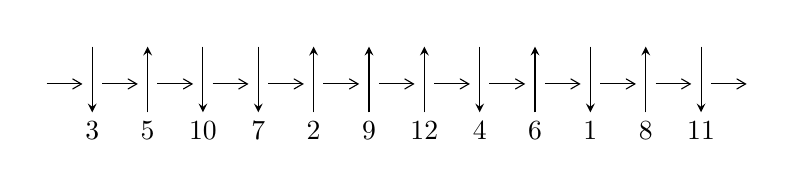
\begin{tikzpicture}[x=20pt, y=17pt]
	% nodes
	\node (C0) at (0, 0) {};
	\node (C1) at (1, 0) {};
	\node (C1U) at (1, +1) {};
	\node (C1D) at (1, -1) {3};

	\node (C2) at (2, 0) {};
	\node (C2U) at (2, +1) {};
	\node (C2D) at (2, -1) {5};

	\node (C3) at (3, 0) {};
	\node (C3U) at (3, +1) {};
	\node (C3D) at (3, -1) {10};

	\node (C4) at (4, 0) {};
	\node (C4U) at (4, +1) {};
	\node (C4D) at (4, -1) {7};

	\node (C5) at (5, 0) {};
	\node (C5U) at (5, +1) {};
	\node (C5D) at (5, -1) {2};

	\node (C6) at (6, 0) {};
	\node (C6U) at (6, +1) {};
	\node (C6D) at (6, -1) {9};

	\node (C7) at (7, 0) {};
	\node (C7U) at (7, +1) {};
	\node (C7D) at (7, -1) {12};

	\node (C8) at (8, 0) {};
	\node (C8U) at (8, +1) {};
	\node (C8D) at (8, -1) {4};

	\node (C9) at (9, 0) {};
	\node (C9U) at (9, +1) {};
	\node (C9D) at (9, -1) {6};

	\node (C10) at (10, 0) {};
	\node (C10U) at (10, +1) {};
	\node (C10D) at (10, -1) {1};

	\node (C11) at (11, 0) {};
	\node (C11U) at (11, +1) {};
	\node (C11D) at (11, -1) {8};

	\node (C12) at (12, 0) {};
	\node (C12U) at (12, +1) {};
	\node (C12D) at (12, -1) {11};
	\node (C13) at (13, 0) {};

	% arrows
	\draw[->,>={angle 60}]
	(C0) edge (C1) (C1) edge (C2) (C2) edge (C3) (C3) edge (C4) (C4) edge (C5) (C5) edge (C6) (C6) edge (C7) (C7) edge (C8) (C8) edge (C9) (C9) edge (C10) (C10) edge (C11) (C11) edge (C12) (C12) edge (C13) ;	\draw[->,>=stealth]
	(C1U) edge (C1D) (C2D) edge (C2U) (C3U) edge (C3D) (C4U) edge (C4D) (C5D) edge (C5U) (C6D) edge (C6U) (C7D) edge (C7U) (C8U) edge (C8D) (C9D) edge (C9U) (C10U) edge (C10D) (C11D) edge (C11U) (C12U) edge (C12D) ;
	\end{tikzpicture} \\
\hhline{~~} \\& 
\textbf{Solving Sequence} \\ \cline{2-2} 
 &
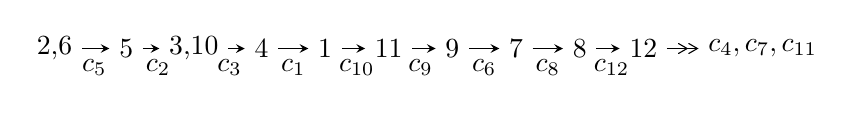
\begin{tikzpicture}[x=23pt, y=7pt]
	% node
	\node (A0) at (-1/8, 0) {2,6};
	\node (A1) at (1, 0) {5};
	\node (A2) at (33/16, 0) {3,10};
	\node (A3) at (25/8, 0) {4};
	\node (A4) at (33/8, 0) {1};
	\node (A5) at (41/8, 0) {11};
	\node (A6) at (49/8, 0) {9};
	\node (A7) at (57/8, 0) {7};
	\node (A8) at (65/8, 0) {8};
	\node (A9) at (73/8, 0) {12};
	\node (C1) at (1/2, -1) {$c_{5}$};
	\node (C2) at (3/2, -1) {$c_{2}$};
	\node (C3) at (21/8, -1) {$c_{3}$};
	\node (C4) at (29/8, -1) {$c_{1}$};
	\node (C5) at (37/8, -1) {$c_{10}$};
	\node (C6) at (45/8, -1) {$c_{9}$};
	\node (C7) at (53/8, -1) {$c_{6}$};
	\node (C8) at (61/8, -1) {$c_{8}$};
	\node (C9) at (69/8, -1) {$c_{12}$};
	\node (A10) at (11, 0) {$c_{4},c_{7},c_{11}$};

	% edge
	\draw[->,>=stealth]	
	(A0) edge (A1) (A1) edge (A2) (A2) edge (A3) (A3) edge (A4) (A4) edge (A5) (A5) edge (A6) (A6) edge (A7) (A7) edge (A8) (A8) edge (A9) ;
	\draw[->>,>={angle 60}]	
	(A9) edge (A10);
\end{tikzpicture} \\ 

\end{tabular} \\

\footnotetext{
The image of knot diagram is generated by the software ``\textbf{Draw programme}" developed by Andrew Bartholomew(\url{http://www.layer8.co.uk/maths/draw/index.htm\#Running-draw}), where we modified some parts for our purpose(\url{https://github.com/CATsTAILs/LinksPainter}).
}\phantom \\ \newline 
\centering \textbf{Ideals for irreducible components\footnotemark of $X_{\text{par}}$} 
 
\begin{align*}
I^u_{1}&=\langle 
4.09817\times10^{213} u^{103}+9.03681\times10^{212} u^{102}+\cdots+3.04803\times10^{213} b+3.78252\times10^{213},\\
\phantom{I^u_{1}}&\phantom{= \langle  }2.98967\times10^{213} u^{103}+1.28932\times10^{213} u^{102}+\cdots+3.04803\times10^{213} a+1.33275\times10^{214},\;u^{104}+u^{103}+\cdots-18 u+1\rangle \\
\\
\end{align*}
\raggedright * 1 irreducible components of $\dim_{\mathbb{C}}=0$, with total 104 representations.\\
\footnotetext{All coefficients of polynomials are rational numbers. But the coefficients are sometimes approximated in decimal forms when there is not enough margin.}
\newpage
\renewcommand{\arraystretch}{1}
\centering \section*{I. $I^u_{1}= \langle 4.10\times10^{213} u^{103}+9.04\times10^{212} u^{102}+\cdots+3.05\times10^{213} b+3.78\times10^{213},\;2.99\times10^{213} u^{103}+1.29\times10^{213} u^{102}+\cdots+3.05\times10^{213} a+1.33\times10^{214},\;u^{104}+u^{103}+\cdots-18 u+1 \rangle$}
\flushleft \textbf{(i) Arc colorings}\\
\begin{tabular}{m{7pt} m{180pt} m{7pt} m{180pt} }
\flushright $a_{2}=$&$\begin{pmatrix}0\\u\end{pmatrix}$ \\
\flushright $a_{6}=$&$\begin{pmatrix}1\\0\end{pmatrix}$ \\
\flushright $a_{5}=$&$\begin{pmatrix}1\\u^2\end{pmatrix}$ \\
\flushright $a_{3}=$&$\begin{pmatrix}u\\u^3+u\end{pmatrix}$ \\
\flushright $a_{10}=$&$\begin{pmatrix}-0.980852 u^{103}-0.423002 u^{102}+\cdots-301.358 u-4.37249\\-1.34453 u^{103}-0.296480 u^{102}+\cdots+28.1294 u-1.24097\end{pmatrix}$ \\
\flushright $a_{4}=$&$\begin{pmatrix}-0.165090 u^{103}+0.388729 u^{102}+\cdots-249.973 u+34.5042\\0.0825240 u^{103}-0.759955 u^{102}+\cdots+9.35599 u-2.04593\end{pmatrix}$ \\
\flushright $a_{1}=$&$\begin{pmatrix}u^3\\u^5+u^3+u\end{pmatrix}$ \\
\flushright $a_{11}=$&$\begin{pmatrix}0.326890 u^{103}-0.407412 u^{102}+\cdots-304.926 u-4.11718\\-0.930552 u^{103}-0.197634 u^{102}+\cdots+25.3578 u-1.01648\end{pmatrix}$ \\
\flushright $a_{9}=$&$\begin{pmatrix}0.363680 u^{103}-0.126522 u^{102}+\cdots-329.487 u-3.13152\\-1.34453 u^{103}-0.296480 u^{102}+\cdots+28.1294 u-1.24097\end{pmatrix}$ \\
\flushright $a_{7}=$&$\begin{pmatrix}1.04068 u^{103}-0.0442496 u^{102}+\cdots+304.110 u-29.6838\\1.60067 u^{103}+0.472640 u^{102}+\cdots-11.4919 u+1.90007\end{pmatrix}$ \\
\flushright $a_{8}=$&$\begin{pmatrix}0.203520 u^{103}+0.306686 u^{102}+\cdots-469.111 u+0.852562\\-1.74430 u^{103}-0.392406 u^{102}+\cdots+35.3865 u-1.76628\end{pmatrix}$ \\
\flushright $a_{12}=$&$\begin{pmatrix}2.18547 u^{103}+1.17719 u^{102}+\cdots+313.496 u-36.3829\\0.863820 u^{103}+0.201308 u^{102}+\cdots-1.30985 u+1.64945\end{pmatrix}$\\&\end{tabular}
\flushleft \textbf{(ii) Obstruction class $= -1$}\\~\\
\flushleft \textbf{(iii) Cusp Shapes $= 3.21119 u^{103}-3.19737 u^{102}+\cdots-71.5495 u+0.533728$}\\~\\
\newpage\renewcommand{\arraystretch}{1}
\flushleft \textbf{(iv) u-Polynomials at the component}\newline \\
\begin{tabular}{m{50pt}|m{274pt}}
Crossings & \hspace{64pt}u-Polynomials at each crossing \\
\hline $$\begin{aligned}c_{1}\end{aligned}$$&$\begin{aligned}
&u^{104}+41 u^{103}+\cdots+124 u+1
\end{aligned}$\\
\hline $$\begin{aligned}c_{2},c_{5}\end{aligned}$$&$\begin{aligned}
&u^{104}+u^{103}+\cdots-18 u+1
\end{aligned}$\\
\hline $$\begin{aligned}c_{3}\end{aligned}$$&$\begin{aligned}
&u^{104}+11 u^{103}+\cdots-231098 u+177923
\end{aligned}$\\
\hline $$\begin{aligned}c_{4}\end{aligned}$$&$\begin{aligned}
&u^{104}+23 u^{103}+\cdots+128 u+41
\end{aligned}$\\
\hline $$\begin{aligned}c_{6},c_{9}\end{aligned}$$&$\begin{aligned}
&u^{104}+5 u^{103}+\cdots+10 u^2+1
\end{aligned}$\\
\hline $$\begin{aligned}c_{7},c_{11}\end{aligned}$$&$\begin{aligned}
&u^{104}-5 u^{103}+\cdots-2 u+1
\end{aligned}$\\
\hline $$\begin{aligned}c_{8}\end{aligned}$$&$\begin{aligned}
&u^{104}+u^{103}+\cdots-10 u+1
\end{aligned}$\\
\hline $$\begin{aligned}c_{10},c_{12}\end{aligned}$$&$\begin{aligned}
&u^{104}+29 u^{103}+\cdots+20 u+1
\end{aligned}$\\
\hline
\end{tabular}\\~\\
\newpage\renewcommand{\arraystretch}{1}
\flushleft \textbf{(v) Riley Polynomials at the component}\newline \\
\begin{tabular}{m{50pt}|m{274pt}}
Crossings & \hspace{64pt}Riley Polynomials at each crossing \\
\hline $$\begin{aligned}c_{1}\end{aligned}$$&$\begin{aligned}
&y^{104}+45 y^{103}+\cdots+126804 y+1
\end{aligned}$\\
\hline $$\begin{aligned}c_{2},c_{5}\end{aligned}$$&$\begin{aligned}
&y^{104}+41 y^{103}+\cdots+124 y+1
\end{aligned}$\\
\hline $$\begin{aligned}c_{3}\end{aligned}$$&$\begin{aligned}
&y^{104}-455 y^{103}+\cdots+1024648387080 y+31656593929
\end{aligned}$\\
\hline $$\begin{aligned}c_{4}\end{aligned}$$&$\begin{aligned}
&y^{104}+425 y^{103}+\cdots+199112 y+1681
\end{aligned}$\\
\hline $$\begin{aligned}c_{6},c_{9}\end{aligned}$$&$\begin{aligned}
&y^{104}+65 y^{103}+\cdots+20 y+1
\end{aligned}$\\
\hline $$\begin{aligned}c_{7},c_{11}\end{aligned}$$&$\begin{aligned}
&y^{104}+29 y^{103}+\cdots+20 y+1
\end{aligned}$\\
\hline $$\begin{aligned}c_{8}\end{aligned}$$&$\begin{aligned}
&y^{104}+5 y^{103}+\cdots-12 y+1
\end{aligned}$\\
\hline $$\begin{aligned}c_{10},c_{12}\end{aligned}$$&$\begin{aligned}
&y^{104}+93 y^{103}+\cdots-4 y+1
\end{aligned}$\\
\hline
\end{tabular}\\~\\
\newpage\flushleft \textbf{(vi) Complex Volumes and Cusp Shapes}
$$\begin{array}{c|c|c}  
\text{Solutions to }I^u_{1}& \I (\text{vol} + \sqrt{-1}CS) & \text{Cusp shape}\\
 \hline 
\begin{aligned}
u &= \phantom{-}0.505387 + 0.862142 I \\
a &= -6.9147 - 13.2965 I \\
b &= -0.015623 + 1.032430 I\end{aligned}
 & \phantom{-}1.40373 - 0.79963 I & \phantom{-0.000000 } 0 \\ \hline\begin{aligned}
u &= \phantom{-}0.505387 - 0.862142 I \\
a &= -6.9147 + 13.2965 I \\
b &= -0.015623 - 1.032430 I\end{aligned}
 & \phantom{-}1.40373 + 0.79963 I & \phantom{-0.000000 } 0 \\ \hline\begin{aligned}
u &= \phantom{-}0.501219 + 0.873062 I \\
a &= \phantom{-}13.51170 + 2.65015 I \\
b &= \phantom{-}0.038652 - 1.005710 I\end{aligned}
 & \phantom{-}1.36834 + 4.88130 I & \phantom{-0.000000 } 0 \\ \hline\begin{aligned}
u &= \phantom{-}0.501219 - 0.873062 I \\
a &= \phantom{-}13.51170 - 2.65015 I \\
b &= \phantom{-}0.038652 + 1.005710 I\end{aligned}
 & \phantom{-}1.36834 - 4.88130 I & \phantom{-0.000000 } 0 \\ \hline\begin{aligned}
u &= \phantom{-}0.996201 + 0.173488 I \\
a &= \phantom{-}0.392374 + 0.187730 I \\
b &= \phantom{-}0.332779 - 0.565610 I\end{aligned}
 & \phantom{-}5.81316 - 2.80924 I & \phantom{-0.000000 } 0 \\ \hline\begin{aligned}
u &= \phantom{-}0.996201 - 0.173488 I \\
a &= \phantom{-}0.392374 - 0.187730 I \\
b &= \phantom{-}0.332779 + 0.565610 I\end{aligned}
 & \phantom{-}5.81316 + 2.80924 I & \phantom{-0.000000 } 0 \\ \hline\begin{aligned}
u &= -0.586727 + 0.827689 I \\
a &= -0.096700 + 1.025660 I \\
b &= \phantom{-}0.81719 + 1.39541 I\end{aligned}
 & \phantom{-}2.94293 + 0.22991 I & \phantom{-0.000000 } 0 \\ \hline\begin{aligned}
u &= -0.586727 - 0.827689 I \\
a &= -0.096700 - 1.025660 I \\
b &= \phantom{-}0.81719 - 1.39541 I\end{aligned}
 & \phantom{-}2.94293 - 0.22991 I & \phantom{-0.000000 } 0 \\ \hline\begin{aligned}
u &= \phantom{-}0.988414 + 0.247276 I \\
a &= -0.405864 - 0.194160 I \\
b &= -0.334041 + 0.546829 I\end{aligned}
 & \phantom{-}5.78547 + 3.15535 I & \phantom{-0.000000 } 0 \\ \hline\begin{aligned}
u &= \phantom{-}0.988414 - 0.247276 I \\
a &= -0.405864 + 0.194160 I \\
b &= -0.334041 - 0.546829 I\end{aligned}
 & \phantom{-}5.78547 - 3.15535 I & \phantom{-0.000000 } 0\\
 \hline 
 \end{array}$$\newpage$$\begin{array}{c|c|c}  
\text{Solutions to }I^u_{1}& \I (\text{vol} + \sqrt{-1}CS) & \text{Cusp shape}\\
 \hline 
\begin{aligned}
u &= -0.836334 + 0.599618 I \\
a &= -1.38843 - 0.45981 I \\
b &= -1.013470 + 0.146587 I\end{aligned}
 & \phantom{-}7.69993 + 7.02828 I & \phantom{-0.000000 } 0 \\ \hline\begin{aligned}
u &= -0.836334 - 0.599618 I \\
a &= -1.38843 + 0.45981 I \\
b &= -1.013470 - 0.146587 I\end{aligned}
 & \phantom{-}7.69993 - 7.02828 I & \phantom{-0.000000 } 0 \\ \hline\begin{aligned}
u &= \phantom{-}0.412346 + 0.942918 I \\
a &= \phantom{-}1.73833 - 2.45352 I \\
b &= \phantom{-}0.123181 + 1.085540 I\end{aligned}
 & -3.31178 + 1.98558 I & \phantom{-0.000000 } 0 \\ \hline\begin{aligned}
u &= \phantom{-}0.412346 - 0.942918 I \\
a &= \phantom{-}1.73833 + 2.45352 I \\
b &= \phantom{-}0.123181 - 1.085540 I\end{aligned}
 & -3.31178 - 1.98558 I & \phantom{-0.000000 } 0 \\ \hline\begin{aligned}
u &= -0.607552 + 0.837105 I \\
a &= \phantom{-}1.37091 + 0.92114 I \\
b &= \phantom{-}1.292200 - 0.191558 I\end{aligned}
 & \phantom{-}3.03222 - 2.39899 I & \phantom{-0.000000 } 0 \\ \hline\begin{aligned}
u &= -0.607552 - 0.837105 I \\
a &= \phantom{-}1.37091 - 0.92114 I \\
b &= \phantom{-}1.292200 + 0.191558 I\end{aligned}
 & \phantom{-}3.03222 + 2.39899 I & \phantom{-0.000000 } 0 \\ \hline\begin{aligned}
u &= -0.581639 + 0.858516 I \\
a &= \phantom{-}2.05036 + 0.18942 I \\
b &= \phantom{-}0.57922 - 1.63420 I\end{aligned}
 & \phantom{-}2.85030 - 4.87673 I & \phantom{-0.000000 } 0 \\ \hline\begin{aligned}
u &= -0.581639 - 0.858516 I \\
a &= \phantom{-}2.05036 - 0.18942 I \\
b &= \phantom{-}0.57922 + 1.63420 I\end{aligned}
 & \phantom{-}2.85030 + 4.87673 I & \phantom{-0.000000 } 0 \\ \hline\begin{aligned}
u &= -0.816116 + 0.645065 I \\
a &= \phantom{-}1.37577 + 0.50366 I \\
b &= \phantom{-}1.033450 - 0.153354 I\end{aligned}
 & \phantom{-}8.39953 + 0.74620 I & \phantom{-0.000000 } 0 \\ \hline\begin{aligned}
u &= -0.816116 - 0.645065 I \\
a &= \phantom{-}1.37577 - 0.50366 I \\
b &= \phantom{-}1.033450 + 0.153354 I\end{aligned}
 & \phantom{-}8.39953 - 0.74620 I & \phantom{-0.000000 } 0\\
 \hline 
 \end{array}$$\newpage$$\begin{array}{c|c|c}  
\text{Solutions to }I^u_{1}& \I (\text{vol} + \sqrt{-1}CS) & \text{Cusp shape}\\
 \hline 
\begin{aligned}
u &= -0.530773 + 0.778902 I \\
a &= -1.99026 - 0.06316 I \\
b &= -0.33699 + 1.68216 I\end{aligned}
 & \phantom{-}2.11332 + 1.88283 I & \phantom{-0.000000 } 0 \\ \hline\begin{aligned}
u &= -0.530773 - 0.778902 I \\
a &= -1.99026 + 0.06316 I \\
b &= -0.33699 - 1.68216 I\end{aligned}
 & \phantom{-}2.11332 - 1.88283 I & \phantom{-0.000000 } 0 \\ \hline\begin{aligned}
u &= -0.843149 + 0.398961 I \\
a &= -0.796579 - 0.889832 I \\
b &= -0.537396 - 1.228480 I\end{aligned}
 & -2.96530 + 7.47434 I & \phantom{-0.000000 } 0 \\ \hline\begin{aligned}
u &= -0.843149 - 0.398961 I \\
a &= -0.796579 + 0.889832 I \\
b &= -0.537396 + 1.228480 I\end{aligned}
 & -2.96530 - 7.47434 I & \phantom{-0.000000 } 0 \\ \hline\begin{aligned}
u &= -0.562569 + 0.913650 I \\
a &= \phantom{-}0.450930 - 0.767392 I \\
b &= -0.67940 - 1.58168 I\end{aligned}
 & \phantom{-}1.65712 - 6.30829 I & \phantom{-0.000000 } 0 \\ \hline\begin{aligned}
u &= -0.562569 - 0.913650 I \\
a &= \phantom{-}0.450930 + 0.767392 I \\
b &= -0.67940 + 1.58168 I\end{aligned}
 & \phantom{-}1.65712 + 6.30829 I & \phantom{-0.000000 } 0 \\ \hline\begin{aligned}
u &= -0.063215 + 1.078180 I \\
a &= -0.386819 - 0.988960 I \\
b &= \phantom{-}0.227112 + 1.304850 I\end{aligned}
 & -5.04325 + 2.34615 I & \phantom{-0.000000 } 0 \\ \hline\begin{aligned}
u &= -0.063215 - 1.078180 I \\
a &= -0.386819 + 0.988960 I \\
b &= \phantom{-}0.227112 - 1.304850 I\end{aligned}
 & -5.04325 - 2.34615 I & \phantom{-0.000000 } 0 \\ \hline\begin{aligned}
u &= -0.953692 + 0.515568 I \\
a &= \phantom{-}0.682831 + 0.711222 I \\
b &= \phantom{-}0.554982 + 1.263190 I\end{aligned}
 & \phantom{-}4.94747 + 6.36433 I & \phantom{-0.000000 } 0 \\ \hline\begin{aligned}
u &= -0.953692 - 0.515568 I \\
a &= \phantom{-}0.682831 - 0.711222 I \\
b &= \phantom{-}0.554982 - 1.263190 I\end{aligned}
 & \phantom{-}4.94747 - 6.36433 I & \phantom{-0.000000 } 0\\
 \hline 
 \end{array}$$\newpage$$\begin{array}{c|c|c}  
\text{Solutions to }I^u_{1}& \I (\text{vol} + \sqrt{-1}CS) & \text{Cusp shape}\\
 \hline 
\begin{aligned}
u &= \phantom{-}0.553236 + 0.727396 I \\
a &= -0.386426 + 0.064707 I \\
b &= -0.101505 + 0.353271 I\end{aligned}
 & \phantom{-}0.11772 + 1.44824 I & \phantom{-0.000000 } 0 \\ \hline\begin{aligned}
u &= \phantom{-}0.553236 - 0.727396 I \\
a &= -0.386426 - 0.064707 I \\
b &= -0.101505 - 0.353271 I\end{aligned}
 & \phantom{-}0.11772 - 1.44824 I & \phantom{-0.000000 } 0 \\ \hline\begin{aligned}
u &= -0.977564 + 0.488443 I \\
a &= -0.721488 - 0.693464 I \\
b &= -0.547978 - 1.264760 I\end{aligned}
 & \phantom{-}4.22367 + 12.57380 I & \phantom{-0.000000 } 0 \\ \hline\begin{aligned}
u &= -0.977564 - 0.488443 I \\
a &= -0.721488 + 0.693464 I \\
b &= -0.547978 + 1.264760 I\end{aligned}
 & \phantom{-}4.22367 - 12.57380 I & \phantom{-0.000000 } 0 \\ \hline\begin{aligned}
u &= \phantom{-}0.161347 + 1.083530 I \\
a &= -0.198232 - 0.559806 I \\
b &= -0.565720 - 0.200757 I\end{aligned}
 & \phantom{-}1.13917 + 6.36070 I & \phantom{-0.000000 } 0 \\ \hline\begin{aligned}
u &= \phantom{-}0.161347 - 1.083530 I \\
a &= -0.198232 + 0.559806 I \\
b &= -0.565720 + 0.200757 I\end{aligned}
 & \phantom{-}1.13917 - 6.36070 I & \phantom{-0.000000 } 0 \\ \hline\begin{aligned}
u &= \phantom{-}0.255973 + 1.066190 I \\
a &= \phantom{-}0.168535 + 0.484109 I \\
b &= \phantom{-}0.497613 + 0.161245 I\end{aligned}
 & \phantom{-}1.62262 + 0.79893 I & \phantom{-0.000000 } 0 \\ \hline\begin{aligned}
u &= \phantom{-}0.255973 - 1.066190 I \\
a &= \phantom{-}0.168535 - 0.484109 I \\
b &= \phantom{-}0.497613 - 0.161245 I\end{aligned}
 & \phantom{-}1.62262 - 0.79893 I & \phantom{-0.000000 } 0 \\ \hline\begin{aligned}
u &= -0.737290 + 0.506701 I \\
a &= \phantom{-}0.594472 + 0.998715 I \\
b &= \phantom{-}0.582907 + 1.204340 I\end{aligned}
 & \phantom{-}0.12101 + 3.83292 I & \phantom{-0.000000 } 0 \\ \hline\begin{aligned}
u &= -0.737290 - 0.506701 I \\
a &= \phantom{-}0.594472 - 0.998715 I \\
b &= \phantom{-}0.582907 - 1.204340 I\end{aligned}
 & \phantom{-}0.12101 - 3.83292 I & \phantom{-0.000000 } 0\\
 \hline 
 \end{array}$$\newpage$$\begin{array}{c|c|c}  
\text{Solutions to }I^u_{1}& \I (\text{vol} + \sqrt{-1}CS) & \text{Cusp shape}\\
 \hline 
\begin{aligned}
u &= \phantom{-}0.397803 + 0.796446 I \\
a &= \phantom{-}2.13538 - 1.07987 I \\
b &= \phantom{-}0.124948 - 0.824931 I\end{aligned}
 & -2.81189 + 1.48523 I & \phantom{-0.000000 } 0 \\ \hline\begin{aligned}
u &= \phantom{-}0.397803 - 0.796446 I \\
a &= \phantom{-}2.13538 + 1.07987 I \\
b &= \phantom{-}0.124948 + 0.824931 I\end{aligned}
 & -2.81189 - 1.48523 I & \phantom{-0.000000 } 0 \\ \hline\begin{aligned}
u &= -0.244913 + 1.089920 I \\
a &= \phantom{-}0.534481 + 0.533393 I \\
b &= -0.27978 - 1.39230 I\end{aligned}
 & -7.44706 - 1.35876 I & \phantom{-0.000000 } 0 \\ \hline\begin{aligned}
u &= -0.244913 - 1.089920 I \\
a &= \phantom{-}0.534481 - 0.533393 I \\
b &= -0.27978 + 1.39230 I\end{aligned}
 & -7.44706 + 1.35876 I & \phantom{-0.000000 } 0 \\ \hline\begin{aligned}
u &= -0.563984 + 0.974977 I \\
a &= -0.967704 - 1.012100 I \\
b &= -1.267190 - 0.108109 I\end{aligned}
 & -1.16734 - 6.56904 I & \phantom{-0.000000 } 0 \\ \hline\begin{aligned}
u &= -0.563984 - 0.974977 I \\
a &= -0.967704 + 1.012100 I \\
b &= -1.267190 + 0.108109 I\end{aligned}
 & -1.16734 + 6.56904 I & \phantom{-0.000000 } 0 \\ \hline\begin{aligned}
u &= \phantom{-}0.563323 + 0.976069 I \\
a &= \phantom{-}0.214860 + 0.203704 I \\
b &= \phantom{-}0.301646 - 0.087160 I\end{aligned}
 & -0.88605 + 3.09648 I & \phantom{-0.000000 } 0 \\ \hline\begin{aligned}
u &= \phantom{-}0.563323 - 0.976069 I \\
a &= \phantom{-}0.214860 - 0.203704 I \\
b &= \phantom{-}0.301646 + 0.087160 I\end{aligned}
 & -0.88605 - 3.09648 I & \phantom{-0.000000 } 0 \\ \hline\begin{aligned}
u &= \phantom{-}0.664866 + 0.555061 I \\
a &= \phantom{-}0.150859 + 0.411065 I \\
b &= \phantom{-}0.197184 + 0.715235 I\end{aligned}
 & \phantom{-}0.20121 + 1.54957 I & \phantom{-0.000000 } 0 \\ \hline\begin{aligned}
u &= \phantom{-}0.664866 - 0.555061 I \\
a &= \phantom{-}0.150859 - 0.411065 I \\
b &= \phantom{-}0.197184 - 0.715235 I\end{aligned}
 & \phantom{-}0.20121 - 1.54957 I & \phantom{-0.000000 } 0\\
 \hline 
 \end{array}$$\newpage$$\begin{array}{c|c|c}  
\text{Solutions to }I^u_{1}& \I (\text{vol} + \sqrt{-1}CS) & \text{Cusp shape}\\
 \hline 
\begin{aligned}
u &= -0.541563 + 1.038640 I \\
a &= -1.92835 - 0.47733 I \\
b &= -0.68081 + 1.34674 I\end{aligned}
 & -5.56704 - 5.39461 I & \phantom{-0.000000 } 0 \\ \hline\begin{aligned}
u &= -0.541563 - 1.038640 I \\
a &= -1.92835 + 0.47733 I \\
b &= -0.68081 - 1.34674 I\end{aligned}
 & -5.56704 + 5.39461 I & \phantom{-0.000000 } 0 \\ \hline\begin{aligned}
u &= -0.139441 + 0.815286 I \\
a &= -0.107784 - 0.995643 I \\
b &= -0.688124 - 0.558770 I\end{aligned}
 & -3.50757 + 1.44378 I & -7.49193 - 4.44049 I \\ \hline\begin{aligned}
u &= -0.139441 - 0.815286 I \\
a &= -0.107784 + 0.995643 I \\
b &= -0.688124 + 0.558770 I\end{aligned}
 & -3.50757 - 1.44378 I & -7.49193 + 4.44049 I \\ \hline\begin{aligned}
u &= \phantom{-}0.791541 + 0.865692 I \\
a &= -0.925362 - 0.291803 I \\
b &= -0.239348 - 0.862721 I\end{aligned}
 & -0.53591 + 3.95919 I & \phantom{-0.000000 } 0 \\ \hline\begin{aligned}
u &= \phantom{-}0.791541 - 0.865692 I \\
a &= -0.925362 + 0.291803 I \\
b &= -0.239348 + 0.862721 I\end{aligned}
 & -0.53591 - 3.95919 I & \phantom{-0.000000 } 0 \\ \hline\begin{aligned}
u &= \phantom{-}0.598103 + 1.032470 I \\
a &= -1.60013 + 0.38394 I \\
b &= -0.209568 - 0.988716 I\end{aligned}
 & -1.29854 + 3.50304 I & \phantom{-0.000000 } 0 \\ \hline\begin{aligned}
u &= \phantom{-}0.598103 - 1.032470 I \\
a &= -1.60013 - 0.38394 I \\
b &= -0.209568 + 0.988716 I\end{aligned}
 & -1.29854 - 3.50304 I & \phantom{-0.000000 } 0 \\ \hline\begin{aligned}
u &= -0.626822 + 1.054980 I \\
a &= \phantom{-}1.86254 + 0.41719 I \\
b &= \phantom{-}0.61435 - 1.37730 I\end{aligned}
 & -1.48010 - 9.03843 I & \phantom{-0.000000 } 0 \\ \hline\begin{aligned}
u &= -0.626822 - 1.054980 I \\
a &= \phantom{-}1.86254 - 0.41719 I \\
b &= \phantom{-}0.61435 + 1.37730 I\end{aligned}
 & -1.48010 + 9.03843 I & \phantom{-0.000000 } 0\\
 \hline 
 \end{array}$$\newpage$$\begin{array}{c|c|c}  
\text{Solutions to }I^u_{1}& \I (\text{vol} + \sqrt{-1}CS) & \text{Cusp shape}\\
 \hline 
\begin{aligned}
u &= \phantom{-}0.786160 + 0.943347 I \\
a &= -0.347310 - 0.183982 I \\
b &= -0.362772 + 0.261162 I\end{aligned}
 & \phantom{-}4.64197 + 0.21423 I & \phantom{-0.000000 } 0 \\ \hline\begin{aligned}
u &= \phantom{-}0.786160 - 0.943347 I \\
a &= -0.347310 + 0.183982 I \\
b &= -0.362772 - 0.261162 I\end{aligned}
 & \phantom{-}4.64197 - 0.21423 I & \phantom{-0.000000 } 0 \\ \hline\begin{aligned}
u &= \phantom{-}0.574664 + 0.511013 I \\
a &= -0.617338 - 0.139145 I \\
b &= -0.206183 + 0.494096 I\end{aligned}
 & \phantom{-}0.254275 + 1.333160 I & \phantom{-}3.09253 - 3.95569 I \\ \hline\begin{aligned}
u &= \phantom{-}0.574664 - 0.511013 I \\
a &= -0.617338 + 0.139145 I \\
b &= -0.206183 - 0.494096 I\end{aligned}
 & \phantom{-}0.254275 - 1.333160 I & \phantom{-}3.09253 + 3.95569 I \\ \hline\begin{aligned}
u &= -0.695804 + 1.019420 I \\
a &= \phantom{-}1.014300 + 0.770211 I \\
b &= \phantom{-}1.146680 + 0.007195 I\end{aligned}
 & \phantom{-}7.25970 - 6.40842 I & \phantom{-0.000000 } 0 \\ \hline\begin{aligned}
u &= -0.695804 - 1.019420 I \\
a &= \phantom{-}1.014300 - 0.770211 I \\
b &= \phantom{-}1.146680 - 0.007195 I\end{aligned}
 & \phantom{-}7.25970 + 6.40842 I & \phantom{-0.000000 } 0 \\ \hline\begin{aligned}
u &= \phantom{-}0.763291 + 0.985949 I \\
a &= \phantom{-}0.335597 + 0.197355 I \\
b &= \phantom{-}0.375401 - 0.234733 I\end{aligned}
 & \phantom{-}4.46281 + 6.08285 I & \phantom{-0.000000 } 0 \\ \hline\begin{aligned}
u &= \phantom{-}0.763291 - 0.985949 I \\
a &= \phantom{-}0.335597 - 0.197355 I \\
b &= \phantom{-}0.375401 + 0.234733 I\end{aligned}
 & \phantom{-}4.46281 - 6.08285 I & \phantom{-0.000000 } 0 \\ \hline\begin{aligned}
u &= \phantom{-}0.098837 + 0.743321 I \\
a &= \phantom{-}1.89127 + 0.34280 I \\
b &= \phantom{-}0.391631 - 0.750203 I\end{aligned}
 & \phantom{-}0.25747 - 2.49818 I & -1.86836 + 3.61739 I \\ \hline\begin{aligned}
u &= \phantom{-}0.098837 - 0.743321 I \\
a &= \phantom{-}1.89127 - 0.34280 I \\
b &= \phantom{-}0.391631 + 0.750203 I\end{aligned}
 & \phantom{-}0.25747 + 2.49818 I & -1.86836 - 3.61739 I\\
 \hline 
 \end{array}$$\newpage$$\begin{array}{c|c|c}  
\text{Solutions to }I^u_{1}& \I (\text{vol} + \sqrt{-1}CS) & \text{Cusp shape}\\
 \hline 
\begin{aligned}
u &= \phantom{-}1.050370 + 0.680338 I \\
a &= \phantom{-}0.563271 + 0.072512 I \\
b &= \phantom{-}0.318996 + 0.781931 I\end{aligned}
 & \phantom{-}5.32160 + 0.40661 I & \phantom{-0.000000 } 0 \\ \hline\begin{aligned}
u &= \phantom{-}1.050370 - 0.680338 I \\
a &= \phantom{-}0.563271 - 0.072512 I \\
b &= \phantom{-}0.318996 - 0.781931 I\end{aligned}
 & \phantom{-}5.32160 - 0.40661 I & \phantom{-0.000000 } 0 \\ \hline\begin{aligned}
u &= -0.687882 + 1.051100 I \\
a &= -0.974401 - 0.763916 I \\
b &= -1.133250 - 0.023746 I\end{aligned}
 & \phantom{-}6.3250 - 12.7173 I & \phantom{-0.000000 } 0 \\ \hline\begin{aligned}
u &= -0.687882 - 1.051100 I \\
a &= -0.974401 + 0.763916 I \\
b &= -1.133250 + 0.023746 I\end{aligned}
 & \phantom{-}6.3250 + 12.7173 I & \phantom{-0.000000 } 0 \\ \hline\begin{aligned}
u &= -0.097678 + 1.256820 I \\
a &= \phantom{-}0.096434 + 0.703259 I \\
b &= -0.307554 - 1.285720 I\end{aligned}
 & -8.65151 + 4.70512 I & \phantom{-0.000000 } 0 \\ \hline\begin{aligned}
u &= -0.097678 - 1.256820 I \\
a &= \phantom{-}0.096434 - 0.703259 I \\
b &= -0.307554 + 1.285720 I\end{aligned}
 & -8.65151 - 4.70512 I & \phantom{-0.000000 } 0 \\ \hline\begin{aligned}
u &= -0.276156 + 0.675129 I \\
a &= -1.84613 - 0.61832 I \\
b &= -0.753175 + 0.632458 I\end{aligned}
 & -0.01020 + 2.19701 I & -2.29099 - 5.45111 I \\ \hline\begin{aligned}
u &= -0.276156 - 0.675129 I \\
a &= -1.84613 + 0.61832 I \\
b &= -0.753175 - 0.632458 I\end{aligned}
 & -0.01020 - 2.19701 I & -2.29099 + 5.45111 I \\ \hline\begin{aligned}
u &= \phantom{-}1.048900 + 0.737652 I \\
a &= -0.604511 - 0.068297 I \\
b &= -0.320223 - 0.798682 I\end{aligned}
 & \phantom{-}5.20836 + 6.36397 I & \phantom{-0.000000 } 0 \\ \hline\begin{aligned}
u &= \phantom{-}1.048900 - 0.737652 I \\
a &= -0.604511 + 0.068297 I \\
b &= -0.320223 + 0.798682 I\end{aligned}
 & \phantom{-}5.20836 - 6.36397 I & \phantom{-0.000000 } 0\\
 \hline 
 \end{array}$$\newpage$$\begin{array}{c|c|c}  
\text{Solutions to }I^u_{1}& \I (\text{vol} + \sqrt{-1}CS) & \text{Cusp shape}\\
 \hline 
\begin{aligned}
u &= -0.625889 + 1.119740 I \\
a &= -1.82121 - 0.45820 I \\
b &= -0.59532 + 1.34507 I\end{aligned}
 & -5.09982 - 12.90830 I & \phantom{-0.000000 } 0 \\ \hline\begin{aligned}
u &= -0.625889 - 1.119740 I \\
a &= -1.82121 + 0.45820 I \\
b &= -0.59532 - 1.34507 I\end{aligned}
 & -5.09982 + 12.90830 I & \phantom{-0.000000 } 0 \\ \hline\begin{aligned}
u &= -0.435139 + 0.541580 I \\
a &= -1.75759 - 0.57039 I \\
b &= -0.843804 + 0.397536 I\end{aligned}
 & -0.03969 + 2.18859 I & \phantom{-0.000000 } 0. - 5.53183 I \\ \hline\begin{aligned}
u &= -0.435139 - 0.541580 I \\
a &= -1.75759 + 0.57039 I \\
b &= -0.843804 - 0.397536 I\end{aligned}
 & -0.03969 - 2.18859 I & \phantom{-0.000000 -}0. + 5.53183 I \\ \hline\begin{aligned}
u &= \phantom{-}0.538328 + 1.211250 I \\
a &= \phantom{-}1.020570 - 0.702140 I \\
b &= \phantom{-}0.269635 + 1.049080 I\end{aligned}
 & -3.27693 + 5.64208 I & \phantom{-0.000000 } 0 \\ \hline\begin{aligned}
u &= \phantom{-}0.538328 - 1.211250 I \\
a &= \phantom{-}1.020570 + 0.702140 I \\
b &= \phantom{-}0.269635 - 1.049080 I\end{aligned}
 & -3.27693 - 5.64208 I & \phantom{-0.000000 } 0 \\ \hline\begin{aligned}
u &= -0.702251 + 1.128830 I \\
a &= \phantom{-}1.77074 + 0.42168 I \\
b &= \phantom{-}0.56556 - 1.35944 I\end{aligned}
 & \phantom{-}3.05623 - 12.40750 I & \phantom{-0.000000 } 0 \\ \hline\begin{aligned}
u &= -0.702251 - 1.128830 I \\
a &= \phantom{-}1.77074 - 0.42168 I \\
b &= \phantom{-}0.56556 + 1.35944 I\end{aligned}
 & \phantom{-}3.05623 + 12.40750 I & \phantom{-0.000000 } 0 \\ \hline\begin{aligned}
u &= -0.699999 + 1.148730 I \\
a &= -1.76232 - 0.43473 I \\
b &= -0.56292 + 1.35286 I\end{aligned}
 & \phantom{-}2.1837 - 18.6708 I & \phantom{-0.000000 } 0 \\ \hline\begin{aligned}
u &= -0.699999 - 1.148730 I \\
a &= -1.76232 + 0.43473 I \\
b &= -0.56292 - 1.35286 I\end{aligned}
 & \phantom{-}2.1837 + 18.6708 I & \phantom{-0.000000 } 0\\
 \hline 
 \end{array}$$\newpage$$\begin{array}{c|c|c}  
\text{Solutions to }I^u_{1}& \I (\text{vol} + \sqrt{-1}CS) & \text{Cusp shape}\\
 \hline 
\begin{aligned}
u &= \phantom{-}0.084454 + 1.345260 I \\
a &= \phantom{-}0.215536 - 0.791522 I \\
b &= \phantom{-}0.312103 + 1.212010 I\end{aligned}
 & -2.26641 + 3.85361 I & \phantom{-0.000000 } 0 \\ \hline\begin{aligned}
u &= \phantom{-}0.084454 - 1.345260 I \\
a &= \phantom{-}0.215536 + 0.791522 I \\
b &= \phantom{-}0.312103 - 1.212010 I\end{aligned}
 & -2.26641 - 3.85361 I & \phantom{-0.000000 } 0 \\ \hline\begin{aligned}
u &= \phantom{-}0.035100 + 1.381650 I \\
a &= -0.180333 + 0.713414 I \\
b &= -0.328473 - 1.223950 I\end{aligned}
 & -2.91423 + 9.64392 I & \phantom{-0.000000 } 0 \\ \hline\begin{aligned}
u &= \phantom{-}0.035100 - 1.381650 I \\
a &= -0.180333 - 0.713414 I \\
b &= -0.328473 + 1.223950 I\end{aligned}
 & -2.91423 - 9.64392 I & \phantom{-0.000000 } 0 \\ \hline\begin{aligned}
u &= \phantom{-}0.570798 + 0.171210 I \\
a &= -0.024673 - 0.218918 I \\
b &= \phantom{-}0.225209 + 0.629606 I\end{aligned}
 & \phantom{-}0.348138 + 1.250510 I & \phantom{-}4.33846 - 5.62577 I \\ \hline\begin{aligned}
u &= \phantom{-}0.570798 - 0.171210 I \\
a &= -0.024673 + 0.218918 I \\
b &= \phantom{-}0.225209 - 0.629606 I\end{aligned}
 & \phantom{-}0.348138 - 1.250510 I & \phantom{-}4.33846 + 5.62577 I \\ \hline\begin{aligned}
u &= -0.512414 + 0.300789 I \\
a &= -0.80972 - 1.57315 I \\
b &= -0.481029 - 1.099690 I\end{aligned}
 & -3.73698 + 1.08033 I & -4.99609 - 1.21844 I \\ \hline\begin{aligned}
u &= -0.512414 - 0.300789 I \\
a &= -0.80972 + 1.57315 I \\
b &= -0.481029 + 1.099690 I\end{aligned}
 & -3.73698 - 1.08033 I & -4.99609 + 1.21844 I \\ \hline\begin{aligned}
u &= \phantom{-}0.74819 + 1.25033 I \\
a &= -0.918808 + 0.360469 I \\
b &= -0.317197 - 0.990579 I\end{aligned}
 & \phantom{-}2.80756 + 3.24354 I & \phantom{-0.000000 } 0 \\ \hline\begin{aligned}
u &= \phantom{-}0.74819 - 1.25033 I \\
a &= -0.918808 - 0.360469 I \\
b &= -0.317197 + 0.990579 I\end{aligned}
 & \phantom{-}2.80756 - 3.24354 I & \phantom{-0.000000 } 0\\
 \hline 
 \end{array}$$\newpage$$\begin{array}{c|c|c}  
\text{Solutions to }I^u_{1}& \I (\text{vol} + \sqrt{-1}CS) & \text{Cusp shape}\\
 \hline 
\begin{aligned}
u &= \phantom{-}0.71866 + 1.28682 I \\
a &= \phantom{-}0.892581 - 0.408496 I \\
b &= \phantom{-}0.321440 + 1.004820 I\end{aligned}
 & \phantom{-}2.50531 + 9.13493 I & \phantom{-0.000000 } 0 \\ \hline\begin{aligned}
u &= \phantom{-}0.71866 - 1.28682 I \\
a &= \phantom{-}0.892581 + 0.408496 I \\
b &= \phantom{-}0.321440 - 1.004820 I\end{aligned}
 & \phantom{-}2.50531 - 9.13493 I & \phantom{-0.000000 } 0 \\ \hline\begin{aligned}
u &= \phantom{-}0.0390323 + 0.0478117 I \\
a &= -15.0554 - 16.4608 I \\
b &= -0.035216 + 1.097540 I\end{aligned}
 & \phantom{-}1.42493 + 2.89189 I & -2.46424 - 2.96057 I \\ \hline\begin{aligned}
u &= \phantom{-}0.0390323 - 0.0478117 I \\
a &= -15.0554 + 16.4608 I \\
b &= -0.035216 - 1.097540 I\end{aligned}
 & \phantom{-}1.42493 - 2.89189 I & -2.46424 + 2.96057 I\\
 \hline 
 \end{array}$$\newpage
\newpage\renewcommand{\arraystretch}{1}
\centering \section*{ II. u-Polynomials}
\begin{tabular}{m{50pt}|m{274pt}}
Crossings & \hspace{64pt}u-Polynomials at each crossing \\
\hline $$\begin{aligned}c_{1}\end{aligned}$$&$\begin{aligned}
&u^{104}+41 u^{103}+\cdots+124 u+1
\end{aligned}$\\
\hline $$\begin{aligned}c_{2},c_{5}\end{aligned}$$&$\begin{aligned}
&u^{104}+u^{103}+\cdots-18 u+1
\end{aligned}$\\
\hline $$\begin{aligned}c_{3}\end{aligned}$$&$\begin{aligned}
&u^{104}+11 u^{103}+\cdots-231098 u+177923
\end{aligned}$\\
\hline $$\begin{aligned}c_{4}\end{aligned}$$&$\begin{aligned}
&u^{104}+23 u^{103}+\cdots+128 u+41
\end{aligned}$\\
\hline $$\begin{aligned}c_{6},c_{9}\end{aligned}$$&$\begin{aligned}
&u^{104}+5 u^{103}+\cdots+10 u^2+1
\end{aligned}$\\
\hline $$\begin{aligned}c_{7},c_{11}\end{aligned}$$&$\begin{aligned}
&u^{104}-5 u^{103}+\cdots-2 u+1
\end{aligned}$\\
\hline $$\begin{aligned}c_{8}\end{aligned}$$&$\begin{aligned}
&u^{104}+u^{103}+\cdots-10 u+1
\end{aligned}$\\
\hline $$\begin{aligned}c_{10},c_{12}\end{aligned}$$&$\begin{aligned}
&u^{104}+29 u^{103}+\cdots+20 u+1
\end{aligned}$\\
\hline
\end{tabular}\newpage\renewcommand{\arraystretch}{1}
\centering \section*{ III. Riley Polynomials}
\begin{tabular}{m{50pt}|m{274pt}}
Crossings & \hspace{64pt}Riley Polynomials at each crossing \\
\hline $$\begin{aligned}c_{1}\end{aligned}$$&$\begin{aligned}
&y^{104}+45 y^{103}+\cdots+126804 y+1
\end{aligned}$\\
\hline $$\begin{aligned}c_{2},c_{5}\end{aligned}$$&$\begin{aligned}
&y^{104}+41 y^{103}+\cdots+124 y+1
\end{aligned}$\\
\hline $$\begin{aligned}c_{3}\end{aligned}$$&$\begin{aligned}
&y^{104}-455 y^{103}+\cdots+1024648387080 y+31656593929
\end{aligned}$\\
\hline $$\begin{aligned}c_{4}\end{aligned}$$&$\begin{aligned}
&y^{104}+425 y^{103}+\cdots+199112 y+1681
\end{aligned}$\\
\hline $$\begin{aligned}c_{6},c_{9}\end{aligned}$$&$\begin{aligned}
&y^{104}+65 y^{103}+\cdots+20 y+1
\end{aligned}$\\
\hline $$\begin{aligned}c_{7},c_{11}\end{aligned}$$&$\begin{aligned}
&y^{104}+29 y^{103}+\cdots+20 y+1
\end{aligned}$\\
\hline $$\begin{aligned}c_{8}\end{aligned}$$&$\begin{aligned}
&y^{104}+5 y^{103}+\cdots-12 y+1
\end{aligned}$\\
\hline $$\begin{aligned}c_{10},c_{12}\end{aligned}$$&$\begin{aligned}
&y^{104}+93 y^{103}+\cdots-4 y+1
\end{aligned}$\\
\hline
\end{tabular}
\vskip 2pc
\end{document}